% !TEX TS-program = pdflatex
% !TEX encoding = UTF-8 Unicode

% This is a simple template for a LaTeX document using the "article" class.
% See "book", "report", "letter" for other types of document.

\documentclass[11pt]{article} % use larger type; default would be 10pt

\usepackage[utf8]{inputenc} % set input encoding (not needed with XeLaTeX)
\usepackage{tikz}
%%% Examples of Article customizations
% These packages are optional, depending whether you want the features they provide.
% See the LaTeX Companion or other references for full information.

%%% PAGE DIMENSIONS
\usepackage{geometry} % to change the page dimensions
\geometry{a4paper} % or letterpaper (US) or a5paper or....
% \geometry{margins=2in} % for example, change the margins to 2 inches all round
% \geometry{landscape} % set up the page for landscape
%   read geometry.pdf for detailed page layout information

\usepackage{graphicx} % support the \includegraphics command and options

% \usepackage[parfill]{parskip} % Activate to begin paragraphs with an empty line rather than an indent

%%% PACKAGES
\usepackage{booktabs} % for much better looking tables
\usepackage{array} % for better arrays (eg matrices) in maths
\usepackage{paralist} % very flexible & customisable lists (eg. enumerate/itemize, etc.)
\usepackage{verbatim} % adds environment for commenting out blocks of text & for better verbatim
\usepackage{subfig} % make it possible to include more than one captioned figure/table in a single float
% These packages are all incorporated in the memoir class to one degree or another...
\usepackage{url}
\usepackage{hyperref}

%%% HEADERS & FOOTERS
\usepackage{fancyhdr} % This should be set AFTER setting up the page geometry
\pagestyle{fancy} % options: empty , plain , fancy
\renewcommand{\headrulewidth}{0pt} % customise the layout...
\lhead{}\chead{}\rhead{}
\lfoot{}\cfoot{\thepage}\rfoot{}

%%% SECTION TITLE APPEARANCE
\usepackage{sectsty}
\allsectionsfont{\sffamily\mdseries\upshape} % (See the fntguide.pdf for font help)
% (This matches ConTeXt defaults)

%%% ToC (table of contents) APPEARANCE
\usepackage[nottoc,notlof,notlot]{tocbibind} % Put the bibliography in the ToC
\usepackage[titles,subfigure]{tocloft} % Alter the style of the Table of Contents
\renewcommand{\cftsecfont}{\rmfamily\mdseries\upshape}
\renewcommand{\cftsecpagefont}{\rmfamily\mdseries\upshape} % No bold!

%%% END Article customizations

%%% The "real" document content comes below...

\usepackage{amsfonts}
\usepackage{amsmath}
\usepackage{amsthm}
\usepackage{amssymb}

\theoremstyle{definition}
\newtheorem*{beispiel}{Beispiel}
\newtheorem{definition}{Definition}
\newtheorem*{bemerkung}{Bemerkung}
\newtheorem*{beweis}{Beweis}
\newtheorem*{ubung}{Übung}

\title{Selbststudium 3}
\author{Florian Lüthi}
%\date{} % Activate to display a given date or no date (if empty),
         % otherwise the current date is printed 

\begin{document}
\maketitle

\section*{Aufgabe 3.9}

Der gegebene Automat aus Abbildung 3.2 hat es nicht mehr auf die kopierten Seiten geschafft, darum sei er hier aus dem Automaten aus Abbildung 3.8 sowie den ersten paar Sätzen auf Seite 63 reverse-engineered. Nennen wir ihn $A$:

\begin{center}
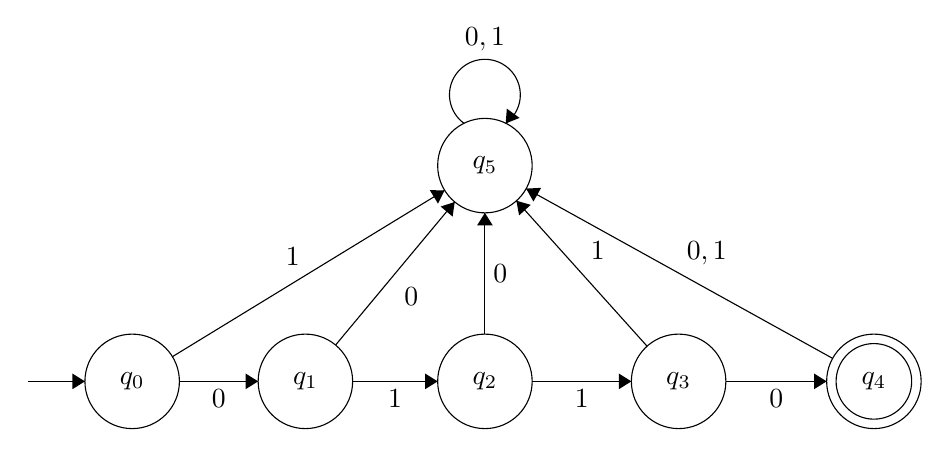
\begin{tikzpicture}[scale=0.2]
\tikzstyle{every node}+=[inner sep=0pt]
\draw [black] (10,-28.3) circle (3);
\draw (10,-28.3) node {$q_0$};
\draw [black] (21,-28.3) circle (3);
\draw (21,-28.3) node {$q_1$};
\draw [black] (32.4,-28.3) circle (3);
\draw (32.4,-28.3) node {$q_2$};
\draw [black] (44.7,-28.3) circle (3);
\draw (44.7,-28.3) node {$q_3$};
\draw [black] (57.1,-28.3) circle (3);
\draw (57.1,-28.3) node {$q_4$};
\draw [black] (57.1,-28.3) circle (2.4);
\draw [black] (32.4,-14.6) circle (3);
\draw (32.4,-14.6) node {$q_5$};
\draw [black] (3.4,-28.3) -- (7,-28.3);
\fill [black] (7,-28.3) -- (6.2,-27.8) -- (6.2,-28.8);
\draw [black] (13,-28.3) -- (18,-28.3);
\fill [black] (18,-28.3) -- (17.2,-27.8) -- (17.2,-28.8);
\draw (15.5,-28.8) node [below] {$0$};
\draw [black] (24,-28.3) -- (29.4,-28.3);
\fill [black] (29.4,-28.3) -- (28.6,-27.8) -- (28.6,-28.8);
\draw (26.7,-28.8) node [below] {$1$};
\draw [black] (35.4,-28.3) -- (41.7,-28.3);
\fill [black] (41.7,-28.3) -- (40.9,-27.8) -- (40.9,-28.8);
\draw (38.55,-28.8) node [below] {$1$};
\draw [black] (47.7,-28.3) -- (54.1,-28.3);
\fill [black] (54.1,-28.3) -- (53.3,-27.8) -- (53.3,-28.8);
\draw (50.9,-28.8) node [below] {$0$};
\draw [black] (32.4,-25.3) -- (32.4,-17.6);
\fill [black] (32.4,-17.6) -- (31.9,-18.4) -- (32.9,-18.4);
\draw (32.9,-21.45) node [right] {$0$};
\draw [black] (42.7,-26.07) -- (34.4,-16.83);
\fill [black] (34.4,-16.83) -- (34.57,-17.76) -- (35.31,-17.09);
\draw (39.09,-19.99) node [right] {$1$};
\draw [black] (31.077,-11.92) arc (234:-54:2.25);
\draw (32.4,-7.35) node [above] {$0,1$};
\fill [black] (33.72,-11.92) -- (34.6,-11.57) -- (33.79,-10.98);
\draw [black] (22.92,-25.99) -- (30.48,-16.91);
\fill [black] (30.48,-16.91) -- (29.59,-17.2) -- (30.35,-17.84);
\draw (27.25,-22.89) node [right] {$0$};
\draw [black] (12.56,-26.73) -- (29.84,-16.17);
\fill [black] (29.84,-16.17) -- (28.9,-16.16) -- (29.42,-17.01);
\draw (20.2,-20.95) node [above] {$1$};
\draw [black] (54.48,-26.84) -- (35.02,-16.06);
\fill [black] (35.02,-16.06) -- (35.48,-16.88) -- (35.97,-16.01);
\draw (46.49,-20.95) node [above] {$0,1$};
\end{tikzpicture}
\end{center}

Die Sprache dieses Automaten ist $L(A) = \{0110\}$. $\Sigma^* = \{0,1\}^*$ zerfällt genau wie in Beispiel 3.6 in folgende Klassen:

\begin{eqnarray*}
\textrm{Klasse}[q_0] &=& \{\varepsilon\} \\
\textrm{Klasse}[q_1] &=& \{0\} \\
\textrm{Klasse}[q_2] &=& \{01\} \\
\textrm{Klasse}[q_3] &=& \{011\} \\
\textrm{Klasse}[q_4] &=& \{0110\} \\
\textrm{Klasse}[q_5] &=& \{x \in \{0,1\}^* | x \textrm{ ist kein Präfix von } 0110 \} \\
\end{eqnarray*}

Wir bauen diesen nun in einen Automaten $A'$ um, so dass $L(A') = \{x \in \{0,1\}^* | x $ ist ein Präfix von $0110\}$. Ausserdem möchten wir die Klassen der Zustände unverändert lassen. Wir überlegen uns den Zusammenhang zwischen den Klassen und den akzeptierenden Zuständen für einen beliebigen Automaten $A$ folgendermassen:
\[
\forall q \in Q_A (\textrm{Klasse}[q] \subseteq L(A) \Rightarrow q \in F_A)
\]

(Der Umkehrschluss würde wohl auch gelten, ist für diese Aufgabe aber nicht wichtig.)

Also muss gelten:
\[
\begin{array}{rclcl}
\textrm{Klasse}[q_0] &=& \{\varepsilon\} &\subseteq& L(A') \Rightarrow q_0 \in F_{A'} \\
\textrm{Klasse}[q_1] &=& \{0\} &\subseteq& L(A') \Rightarrow q_1 \in F_{A'}  \\
\textrm{Klasse}[q_2] &=& \{01\} &\subseteq& L(A') \Rightarrow q_2 \in F_{A'}  \\
\textrm{Klasse}[q_3] &=& \{011\} &\subseteq& L(A') \Rightarrow q_3 \in F_{A'}  \\
\textrm{Klasse}[q_4] &=& \{0110\} &\subseteq& L(A') \Rightarrow q_4 \in F_{A'}  \\
\textrm{Klasse}[q_5] &=& \{x \in \{0,1\}^* | x \textrm{ ist kein Präfix von } 0110 \} &\not\subseteq& L(A') \Rightarrow q_5 \notin F_{A'}  \\
\end{array}
\]

Dies bringt uns zur Erkenntnis, dass der einzig nötige Umbau die akzeptierenden Zustände betrifft:

\begin{center}
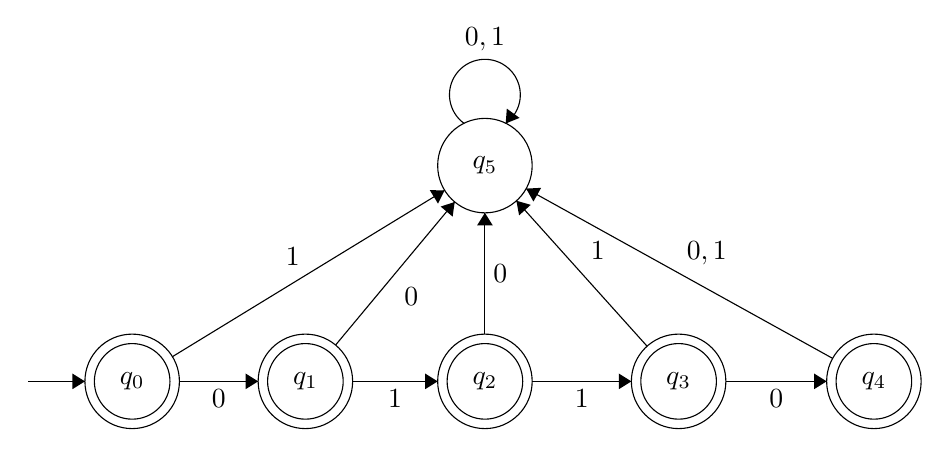
\begin{tikzpicture}[scale=0.2]
\tikzstyle{every node}+=[inner sep=0pt]
\draw [black] (10,-28.3) circle (3);
\draw (10,-28.3) node {$q_0$};
\draw [black] (10,-28.3) circle (2.4);
\draw [black] (21,-28.3) circle (3);
\draw (21,-28.3) node {$q_1$};
\draw [black] (21,-28.3) circle (2.4);
\draw [black] (32.4,-28.3) circle (3);
\draw (32.4,-28.3) node {$q_2$};
\draw [black] (32.4,-28.3) circle (2.4);
\draw [black] (44.7,-28.3) circle (3);
\draw (44.7,-28.3) node {$q_3$};
\draw [black] (44.7,-28.3) circle (2.4);
\draw [black] (57.1,-28.3) circle (3);
\draw (57.1,-28.3) node {$q_4$};
\draw [black] (57.1,-28.3) circle (2.4);
\draw [black] (32.4,-14.6) circle (3);
\draw (32.4,-14.6) node {$q_5$};
\draw [black] (3.4,-28.3) -- (7,-28.3);
\fill [black] (7,-28.3) -- (6.2,-27.8) -- (6.2,-28.8);
\draw [black] (13,-28.3) -- (18,-28.3);
\fill [black] (18,-28.3) -- (17.2,-27.8) -- (17.2,-28.8);
\draw (15.5,-28.8) node [below] {$0$};
\draw [black] (24,-28.3) -- (29.4,-28.3);
\fill [black] (29.4,-28.3) -- (28.6,-27.8) -- (28.6,-28.8);
\draw (26.7,-28.8) node [below] {$1$};
\draw [black] (35.4,-28.3) -- (41.7,-28.3);
\fill [black] (41.7,-28.3) -- (40.9,-27.8) -- (40.9,-28.8);
\draw (38.55,-28.8) node [below] {$1$};
\draw [black] (47.7,-28.3) -- (54.1,-28.3);
\fill [black] (54.1,-28.3) -- (53.3,-27.8) -- (53.3,-28.8);
\draw (50.9,-28.8) node [below] {$0$};
\draw [black] (32.4,-25.3) -- (32.4,-17.6);
\fill [black] (32.4,-17.6) -- (31.9,-18.4) -- (32.9,-18.4);
\draw (32.9,-21.45) node [right] {$0$};
\draw [black] (42.7,-26.07) -- (34.4,-16.83);
\fill [black] (34.4,-16.83) -- (34.57,-17.76) -- (35.31,-17.09);
\draw (39.09,-19.99) node [right] {$1$};
\draw [black] (31.077,-11.92) arc (234:-54:2.25);
\draw (32.4,-7.35) node [above] {$0,1$};
\fill [black] (33.72,-11.92) -- (34.6,-11.57) -- (33.79,-10.98);
\draw [black] (22.92,-25.99) -- (30.48,-16.91);
\fill [black] (30.48,-16.91) -- (29.59,-17.2) -- (30.35,-17.84);
\draw (27.25,-22.89) node [right] {$0$};
\draw [black] (12.56,-26.73) -- (29.84,-16.17);
\fill [black] (29.84,-16.17) -- (28.9,-16.16) -- (29.42,-17.01);
\draw (20.2,-20.95) node [above] {$1$};
\draw [black] (54.48,-26.84) -- (35.02,-16.06);
\fill [black] (35.02,-16.06) -- (35.48,-16.88) -- (35.97,-16.01);
\draw (46.49,-20.95) node [above] {$0,1$};
\end{tikzpicture}
\end{center}

\section*{Aufgabe 3.10}

Hier der (zugegebenermassen nicht sehr phantasievolle) Automat $A$:

\begin{center}
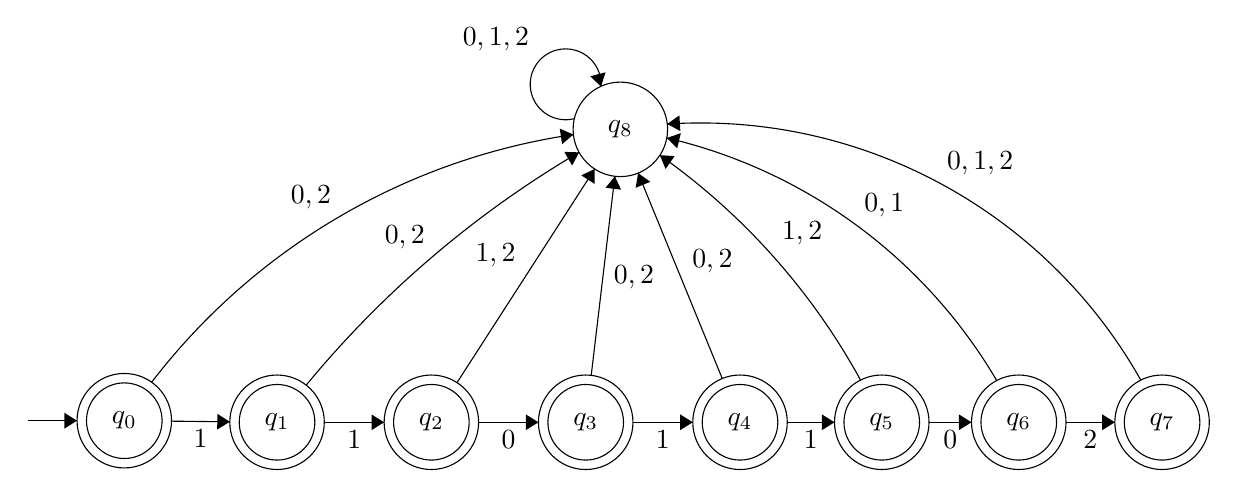
\begin{tikzpicture}[scale=0.2]
\tikzstyle{every node}+=[inner sep=0pt]
\draw [black] (8.3,-25.7) circle (3);
\draw (8.3,-25.7) node {$q_0$};
\draw [black] (8.3,-25.7) circle (2.4);
\draw [black] (18,-25.8) circle (3);
\draw (18,-25.8) node {$q_1$};
\draw [black] (18,-25.8) circle (2.4);
\draw [black] (27.8,-25.8) circle (3);
\draw (27.8,-25.8) node {$q_2$};
\draw [black] (27.8,-25.8) circle (2.4);
\draw [black] (37.6,-25.8) circle (3);
\draw (37.6,-25.8) node {$q_3$};
\draw [black] (37.6,-25.8) circle (2.4);
\draw [black] (47.4,-25.8) circle (3);
\draw (47.4,-25.8) node {$q_4$};
\draw [black] (47.4,-25.8) circle (2.4);
\draw [black] (56.4,-25.8) circle (3);
\draw (56.4,-25.8) node {$q_5$};
\draw [black] (56.4,-25.8) circle (2.4);
\draw [black] (65.1,-25.8) circle (3);
\draw (65.1,-25.8) node {$q_6$};
\draw [black] (65.1,-25.8) circle (2.4);
\draw [black] (74.2,-25.8) circle (3);
\draw (74.2,-25.8) node {$q_7$};
\draw [black] (74.2,-25.8) circle (2.4);
\draw [black] (39.8,-7.2) circle (3);
\draw (39.8,-7.2) node {$q_8$};
\draw [black] (2.2,-25.7) -- (5.3,-25.7);
\fill [black] (5.3,-25.7) -- (4.5,-25.2) -- (4.5,-26.2);
\draw [black] (11.3,-25.73) -- (15,-25.77);
\fill [black] (15,-25.77) -- (14.21,-25.26) -- (14.2,-26.26);
\draw (13.15,-26.26) node [below] {$1$};
\draw [black] (21,-25.8) -- (24.8,-25.8);
\fill [black] (24.8,-25.8) -- (24,-25.3) -- (24,-26.3);
\draw (22.9,-26.3) node [below] {$1$};
\draw [black] (30.8,-25.8) -- (34.6,-25.8);
\fill [black] (34.6,-25.8) -- (33.8,-25.3) -- (33.8,-26.3);
\draw (32.7,-26.3) node [below] {$0$};
\draw [black] (40.6,-25.8) -- (44.4,-25.8);
\fill [black] (44.4,-25.8) -- (43.6,-25.3) -- (43.6,-26.3);
\draw (42.5,-26.3) node [below] {$1$};
\draw [black] (50.4,-25.8) -- (53.4,-25.8);
\fill [black] (53.4,-25.8) -- (52.6,-25.3) -- (52.6,-26.3);
\draw (51.9,-26.3) node [below] {$1$};
\draw [black] (59.4,-25.8) -- (62.1,-25.8);
\fill [black] (62.1,-25.8) -- (61.3,-25.3) -- (61.3,-26.3);
\draw (60.75,-26.3) node [below] {$0$};
\draw [black] (68.1,-25.8) -- (71.2,-25.8);
\fill [black] (71.2,-25.8) -- (70.4,-25.3) -- (70.4,-26.3);
\draw (69.65,-26.3) node [below] {$2$};
\draw [black] (10.038,-23.256) arc (142.50084:98.35073:41.319);
\fill [black] (36.82,-7.53) -- (35.95,-7.15) -- (36.1,-8.14);
\draw (20.15,-12.28) node [above] {$0,2$};
\draw [black] (19.853,-23.441) arc (140.52373:120.41862:65.238);
\fill [black] (37.18,-8.66) -- (36.24,-8.63) -- (36.74,-9.5);
\draw (26.11,-14.8) node [above] {$0,2$};
\draw [black] (29.43,-23.28) -- (38.17,-9.72);
\fill [black] (38.17,-9.72) -- (37.32,-10.12) -- (38.16,-10.66);
\draw (33.18,-15.19) node [left] {$1,2$};
\draw [black] (37.95,-22.82) -- (39.45,-10.18);
\fill [black] (39.45,-10.18) -- (38.86,-10.91) -- (39.85,-11.03);
\draw (39.36,-16.62) node [right] {$0,2$};
\draw [black] (46.27,-23.02) -- (40.93,-9.98);
\fill [black] (40.93,-9.98) -- (40.77,-10.91) -- (41.7,-10.53);
\draw (44.34,-15.59) node [right] {$0,2$};
\draw [black] (42.31,-8.842) arc (54.7755:28.72061:42.449);
\fill [black] (42.31,-8.84) -- (42.67,-9.71) -- (43.25,-8.9);
\draw (50.04,-13.8) node [right] {$1,2$};
\draw [black] (42.749,-7.746) arc (76.90445:30.45054:32.967);
\fill [black] (42.75,-7.75) -- (43.41,-8.41) -- (43.64,-7.44);
\draw (56.56,-12.8) node [above] {$0,1$};
\draw [black] (42.78,-6.863) arc (93.7785:29.42153:32.095);
\fill [black] (42.78,-6.86) -- (43.61,-7.31) -- (43.55,-6.31);
\draw (62.65,-10.15) node [above] {$0,1,2$};
\draw [black] (36.891,-6.517) arc (284.52754:-3.47246:2.25);
\draw (34.03,-1.48) node [left] {$0,1,2$};
\fill [black] (38.57,-4.48) -- (38.86,-3.58) -- (37.89,-3.83);
\end{tikzpicture}
\end{center}

Bestimmen wir die Klassen:

\[
\begin{array}{rclcl}
\textrm{Klasse}[q_0] &=& \{ \varepsilon \} &\subseteq& L(A) \\
\textrm{Klasse}[q_1] &=& \{ 1 \} &\subseteq& L(A) \\
\textrm{Klasse}[q_2] &=& \{ 11 \} &\subseteq& L(A) \\
\textrm{Klasse}[q_3] &=& \{110 \} &\subseteq& L(A) \\
\textrm{Klasse}[q_4] &=& \{ 1101 \} &\subseteq& L(A) \\
\textrm{Klasse}[q_5] &=& \{ 11011 \} &\subseteq& L(A) \\
\textrm{Klasse}[q_6] &=& \{ 110110 \} &\subseteq& L(A) \\
\textrm{Klasse}[q_7] &=& \{ 1101102 \} &\subseteq& L(A) \\
\textrm{Klasse}[q_8] &=& \{ 0,1,2 \}^* - \{\varepsilon, 1, 11, 110, 1101, 11011, 110110, 1101102 \} \\
&=& \{ w \in \{0,1,2\}^* | w \textrm{ ist kein Präfix von } 1101102 \} &\not\subseteq& L(A)

\end{array}
\]

Daraus ergeben sich die akzeptierenden Zustände $F_A = \{q_0, q_1, q_2, q_3, q_4, q_5, q_6, q_7 \}$.

\begin{proof}[Beweis der Korrektheit]
Wir beweisen das, indem wir je ein Wort $x_i$ und $x_j$ aus jeder Klasse nehmen und dann paarweise kombinieren. Dann suchen wir uns für alle Paare ein Wort $z$, sodass gilt:
\[
(x_iz \in L(A) \land x_jz \notin L(A)) \lor (x_iz \notin L(A) \land x_jz \in L(A)).
\]

Wir könnten das jetzt systematisch durchführen, das führt aber zu ziemlich vielen Kombinationen. Einfacher ist es, wenn wir es uns schnell überlegen, weil ja der besprochene Automat einigermassen systematisch ist.

Also: Für die Paare $(x_i, x_j) \in \{ (x_0, x_1), (x_0, x_2), \dots, (x_0, x_7), \dots, (x_6, x_7) \}$ kann $z$ so gewählt werden, dass gilt $x_iz = 1101102$. Dadurch gilt immer $x_iz \in L(A)$ und $x_jz \notin L(A)$ (weil $x_j$ immer um ein Zeichen länger ist als $x_i$, $x_i$ selber aber schon das längste akzeptierte Wort überhaupt ist).

Bleiben noch die Paare $(x_i, x_j) \in \{ (x_1, x_8), (x_2, x_8), \dots, (x_7, x_8) \}$. Hierbei genügt es, jeweils $z = \varepsilon$ zu wählen, weil für alle $x_i \in \{ x_1, \dots x_7 \}$ gelten muss $x_i\varepsilon \in L(A)$ und $x_8 \notin L(A)$.
\end{proof}

\section*{Teilaufgabe 7.4(g)}

\begin{proof}[Beweis]
Wir argumentieren, dass wir mindestens 4 Zustandsklassen benötigen und darum auch mindestens 4 Zustände. Wir beweisen das, indem wir 4 Wörter aus $\{a,b\}^*$ wählen und dann zeigen, dass keine zwei dieser Wörter in derselben Zustandsklasse liegen.

Wir wählen die Wörter:
\begin{eqnarray*}
x_1 &=& \varepsilon \\
x_2 &=& a \\
x_3 &=& aa \\
x_4 &=& aaa
\end{eqnarray*}

Da wir allerdings die Zustandsklassen nicht kennen, können wir nur zeigen, dass für jedes Wort $x$ entweder $x \in L$ oder $x \notin L$ gilt, und dann für alle Paare $(x_i, x_j)$ gilt, dass entweder $x_i \in L$ oder $x_j \in L$ (aber nicht beide gleichzeitig). Dies wird nicht möglich sein zu zeigen. Allerdings wissen wir, dass wenn wir ein Wort $z$ finden und dann gilt: $x_iz \in L \land x_jz \notin L$ (oder umgekehrt), die Zustandsklassen von $x_i$ und $x_j$ äquivalenterweise ebenso unterschiedlich sein müssen (weil sich der Automat ja nicht merken kann, woher er gekommen ist). Also:

\begin{itemize}

\item $(x_1, x_2)$. Wir wählen $z = \varepsilon$ und bekommen:
\begin{eqnarray*}
x_1z = \varepsilon\varepsilon = \varepsilon &\notin& L \\
x_2z = a\varepsilon = a &\in& L \Rightarrow \textrm{Cool.}
\end{eqnarray*}
\item $(x_1, x_3)$. Wir wählen $z = aa$ und bekommen:
\begin{eqnarray*}
x_1z = \varepsilon aa = aa &\notin& L \\
x_3z = aa\cdot aa = aaaa &\in& L \Rightarrow \textrm{Ausgezeichnet.} 
\end{eqnarray*}

\item $(x_1, x_4)$. Wir wählen $z = \varepsilon$ und bekommen:
\begin{eqnarray*}
x_1z = \varepsilon\varepsilon = \varepsilon &\notin& L \\
x_4z = aaa\varepsilon = aaa &\in& L \Rightarrow \textrm{Hervorragend.} 
\end{eqnarray*}

\item $(x_2, x_3)$. Wir wählen $z = \varepsilon$ und bekommen:
\begin{eqnarray*}
x_2z = a\varepsilon = a &\in& L \\
x_3z = aa\varepsilon = aa &\notin& L \Rightarrow \textrm{Extraordinär.} 
\end{eqnarray*}

\item $(x_2, x_4)$. Wir wählen $z =a$ und bekommen:
\begin{eqnarray*}
x_2z = a\cdot a = aa &\notin& L \\
x_4z = aaa\cdot a = aaaa &\in& L \Rightarrow \textrm{Phantastisch.} 
\end{eqnarray*}

\item $(x_3, x_4)$. Wir wählen $z =\varepsilon$ und bekommen:
\begin{eqnarray*}
x_3z = aa\varepsilon = aa &\notin& L \\
x_4z = aaa\cdot \varepsilon = aaa &\in& L \Rightarrow \textrm{Hinreissend.}
\end{eqnarray*}

\end{itemize}

Weil nun kein Paar der vier Wörter $x_1, x_2, x_3, x_4$ zur selben Zustandsklasse gehört, muss es mindestens 4 Zustandsklassen geben und darum auch mindestens vier verschiedene Zustände.
\end{proof}

\section*{Teilaufgabe 7.5(c)}

Konstruieren wir einen solchen Automaten mit Hilfe der Intuition:


\begin{center}
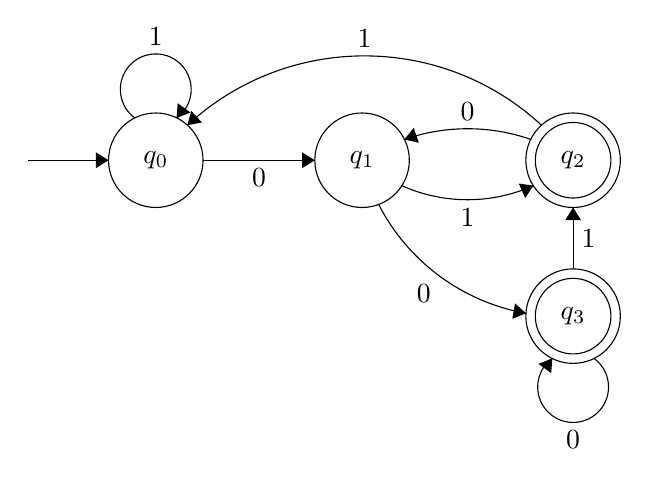
\begin{tikzpicture}[scale=0.2]
\tikzstyle{every node}+=[inner sep=0pt]
\draw [black] (27,-20.7) circle (3);
\draw (27,-20.7) node {$q_1$};
\draw [black] (13.9,-20.7) circle (3);
\draw (13.9,-20.7) node {$q_0$};
\draw [black] (40.4,-20.7) circle (3);
\draw (40.4,-20.7) node {$q_2$};
\draw [black] (40.4,-20.7) circle (2.4);
\draw [black] (40.4,-30.6) circle (3);
\draw (40.4,-30.6) node {$q_3$};
\draw [black] (40.4,-30.6) circle (2.4);
\draw [black] (16.9,-20.7) -- (24,-20.7);
\fill [black] (24,-20.7) -- (23.2,-20.2) -- (23.2,-21.2);
\draw (20.45,-21.2) node [below] {$0$};
\draw [black] (37.882,-22.311) arc (-65.80311:-114.19689:10.204);
\fill [black] (37.88,-22.31) -- (36.95,-22.18) -- (37.36,-23.1);
\draw (33.7,-23.71) node [below] {$1$};
\draw [black] (12.577,-18.02) arc (234:-54:2.25);
\draw (13.9,-13.45) node [above] {$1$};
\fill [black] (15.22,-18.02) -- (16.1,-17.67) -- (15.29,-17.08);
\draw [black] (29.685,-19.378) arc (109.18234:70.81766:12.22);
\fill [black] (29.68,-19.38) -- (30.6,-19.59) -- (30.28,-18.64);
\draw (33.7,-18.2) node [above] {$0$};
\draw [black] (15.906,-18.475) arc (132.76626:47.23374:16.559);
\fill [black] (15.91,-18.48) -- (16.83,-18.3) -- (16.15,-17.56);
\draw (27.15,-13.57) node [above] {$1$};
\draw [black] (5.8,-20.7) -- (10.9,-20.7);
\fill [black] (10.9,-20.7) -- (10.1,-20.2) -- (10.1,-21.2);
\draw [black] (37.412,-30.418) arc (-100.04924:-152.86518:13.084);
\fill [black] (37.41,-30.42) -- (36.71,-29.79) -- (36.54,-30.77);
\draw (30.92,-28.56) node [below] {$0$};
\draw [black] (41.723,-33.28) arc (54:-234:2.25);
\draw (40.4,-37.85) node [below] {$0$};
\fill [black] (39.08,-33.28) -- (38.2,-33.63) -- (39.01,-34.22);
\draw [black] (40.4,-27.6) -- (40.4,-23.7);
\fill [black] (40.4,-23.7) -- (39.9,-24.5) -- (40.9,-24.5);
\draw (40.9,-25.65) node [right] {$1$};
\end{tikzpicture}
\end{center}

Da wir es geschafft haben, einen Automaten mit 4 Zuständen zu konstruieren, und uns für sehr clever halten, behaupten wir, dass man mindestens 4 Zustände braucht, und zwar beweisen wir das mit derselben Kausalkette wie in der oberen Aufgabe.

\begin{proof}[Beweis]
Die Wörter seien $x_1 = 1, x_2 = 10, x_3 = 100, x_4 = 1001$.

\begin{itemize}
\item $(x_1, x_2)$: Wir wählen $z = 1$. $x_1z = 11 \notin L$, $x_2z = 101 \in L$.
\item $(x_1, x_3)$: Wir wählen $z = 1$. $x_1z = 11 \notin L$, $x_3z = 1001 \in L$.
\item $(x_1, x_4)$: Wir wählen $z = \varepsilon$. $x_1z = 1 \notin L$, $x_4z = 1001 \in L$.
\item $(x_2, x_3)$: Wir wählen $z = \varepsilon$. $x_2z = 10 \notin L$, $x_3z = 100 \in L$.
\item $(x_2, x_4)$: Wir wählen $z = \varepsilon$. $x_2z = 10 \notin L$, $x_4z = 1001 \in L$.
\item $(x_3, x_4)$: Wir wählen $z = 0$. $x_3z = 100 \in L$, $x_4z = 10010 \notin L$.
\end{itemize}
\end{proof}

\section*{Aufgabe 7.8}

\begin{proof}[Beweis]
Wir betrachten die unendliche Folge von Wörtern
\[
x_1 = 0, x_2 = 00, x_3 = 000, x_4 = 0000, \dots, x_n = 0^n.
\]
Seien $x_i$ und $x_j$ zwei beliebige Wörter aus dieser Folge ($i \neq j$). Versuchen wir den Beweis auf obige Art, enden wir mit einem Wort
\[
z = 1^{2i},
\]
womit wir erreichen, dass
\[
x_iz = 0^i1^{2i} \in L \textrm{ und } x_jz = 0^j1^{2i} \notin L.
\]
Dadurch sehen wir, jedes Wortpaar $(x_i, x_j)$ mit $i \neq j$ zu zwei verschiedenen Zustandsklassen führt (weil die zugrundeliegende Folge unendlich ist und es darum auch unendlich viele $i$s und $j$s gibt). Dadurch hat jeder Automat, der $L$ akzeptieren soll, unendlich viele Zustände, und darum ist $L$ nicht regulär.
\end{proof}

\end{document}
